%----------------------------------------------------------------------------------------
%       PACKAGES AND THEMES
%
% docs: https://en.wikibooks.org/wiki/LaTeX/Presentations#Introductory_example
%----------------------------------------------------------------------------------------


\documentclass{beamer}

\mode<presentation> {

% The Beamer class comes with a number of default slide themes
% which change the colors and layouts of slides. Below this is a list
% of all the themes, uncomment each in turn to see what they look like.

%\usetheme{default}
%\usetheme{AnnArbor}
%\usetheme{Antibes}
%\usetheme{Bergen}
%\usetheme{Berkeley}
%\usetheme{Berlin}
%\usetheme{Boadilla}
%\usetheme{CambridgeUS}
%\usetheme{Copenhagen}
%\usetheme{Darmstadt}
%\usetheme{Dresden}
\usetheme{Frankfurt}
%\usetheme{Goettingen}
%\usetheme{Hannover}
%\usetheme{Ilmenau}
%\usetheme{JuanLesPins}
%\usetheme{Luebeck}
%\usetheme{Madrid}
%\usetheme{Malmoe}
%\usetheme{Marburg}
%\usetheme{Montpellier}
%\usetheme{PaloAlto}
%\usetheme{Pittsburgh}
%\usetheme{Rochester}
%\usetheme{Singapore}
%\usetheme{Szeged}
%\usetheme{Warsaw}

% As well as themes, the Beamer class has a number of color themes
% for any slide theme. Uncomment each of these in turn to see how it
% changes the colors of your current slide theme.

%\usecolortheme{albatross}
%\usecolortheme{beaver}
%\usecolortheme{beetle}
%\usecolortheme{crane}
%\usecolortheme{dolphin}
%\usecolortheme{dove}
%\usecolortheme{fly}
%\usecolortheme{lily}
%\usecolortheme{orchid}
%\usecolortheme{rose}
%\usecolortheme{seagull}
%\usecolortheme{seahorse}
%\usecolortheme{whale}
%\usecolortheme{wolverine}

%\setbeamertemplate{footline} % To remove the footer line in all slides uncomment this line
%\setbeamertemplate{footline}[page number] % To replace the footer line in all slides with a simple slide count uncomment this line

%\setbeamertemplate{navigation symbols}{} % To remove the navigation symbols from the bottom of all slides uncomment this line
}

%\usepackage[german]{babel}
\usepackage[latin1]{inputenc}
\usepackage{alltt}
\usepackage{beamerthemesplit}

\usepackage{graphicx} % Allows including images
\usepackage{booktabs} % Allows the use of \toprule, \midrule and \bottomrule in tables

\usepackage{color}
\usepackage{listings}
\lstset{
  %basicstyle=\ttfamily\bfseries,
  basicstyle=\ttfamily\footnotesize,
  commentstyle=\color{red}\itshape,
  stringstyle=\color{green},
  showstringspaces=false,
  keywordstyle=\color{blue}\bfseries,
  numberstyle=\ttfamily\tiny,
  frame=single,
  numbers=left,
  numbersep=1em,
  xleftmargin=2em,
  language=Python,
  breaklines=true,
  breakatwhitespace=true,
  postbreak=\hbox{$\hookrightarrow$ },
  showstringspaces=false,
  tabsize=2
}



%% Title Page

\title{Birdhouse Architecture}
%\subtitle{subtitle}
\author{
Carsten Ehbrecht\\
\medskip
{\scriptsize \url{ehbrecht@dkrz.de}}
}
\institute{German Climate Computing Center (DKRZ)}
\date{October 2015}
\subject{Climate Science, Web Processing Service}

% page numbers
%\insertframenumber

% don't count title page
%\addtocounter{framenumber}{-1}


%------------------------------------------------

\begin{document}

%------------------------------------------------

  \begin{frame}[plain]
    \titlepage
  \end{frame}

%------------------------------------------------

  %\AtBeginSection[]
  \AtBeginSection[]{\frame{\frametitle{Overview}\tableofcontents[current]}}
  {
    \begin{frame} % shrink
      \frametitle{Outline}
      \tableofcontents[subsectionstyle=hide/hide]
    \end{frame}
  }

%------------------------------------------------

  \section{Motivation}

  \begin{frame}
    \frametitle{Web Processing Service}
    A web service interface to standardize the way that algorithms are made available on the Internet
    \begin{figure}
      \includegraphics[width=7cm]{images/Wps.png}
    \end{figure}
  \end{frame}

%------------------------------------------------

  \begin{frame}
    \frametitle{WPS Use Case}
    \begin{figure}
      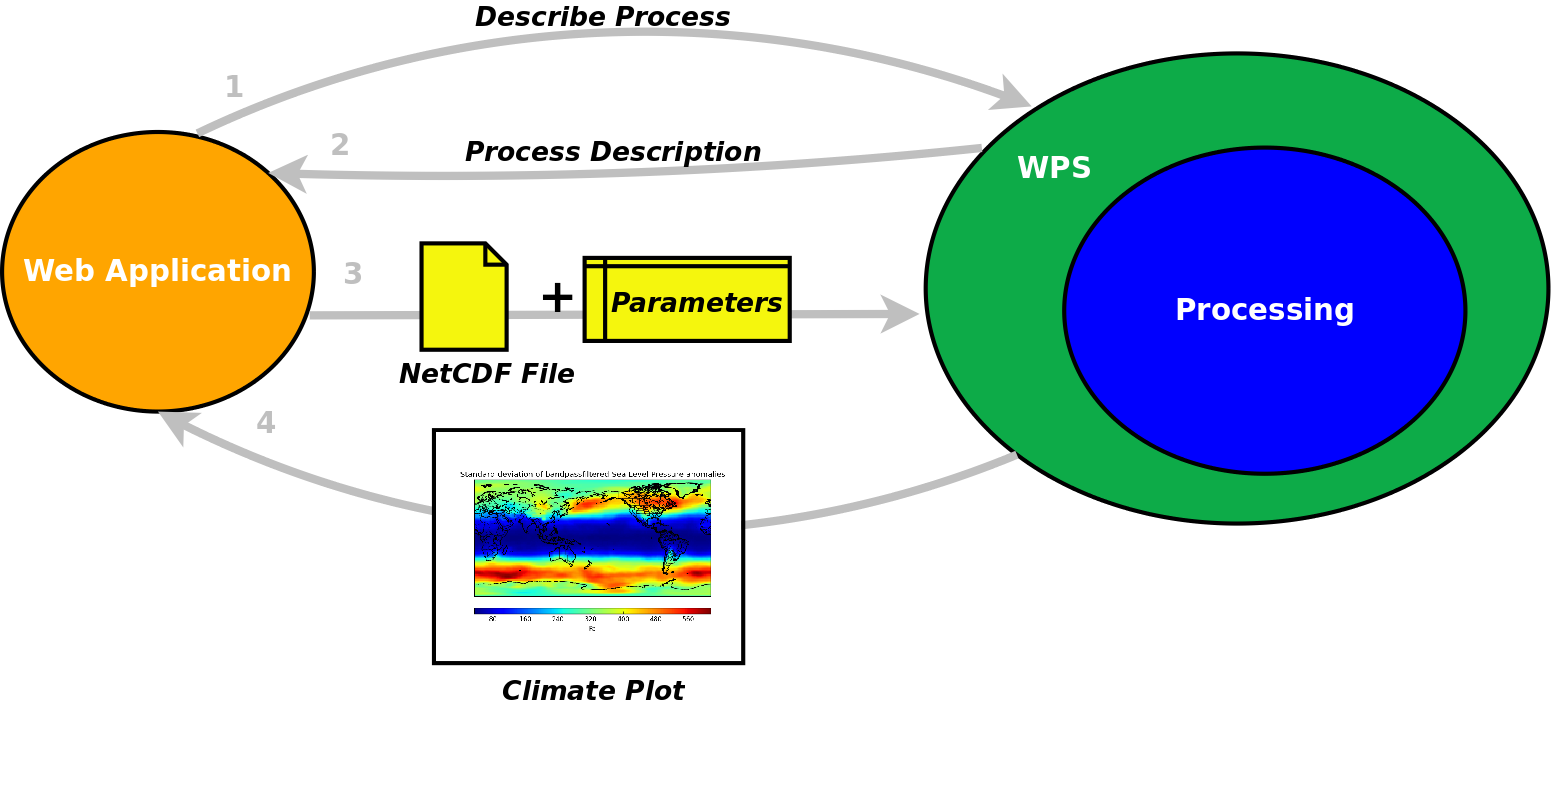
\includegraphics[width=11.5cm]{images/WpsUseCase.png}
    \end{figure}
  \end{frame}


%------------------------------------------------

  \begin{frame}
    \frametitle{What does WPS provide?}
    \begin{itemize}
      \item web access to your algorithms (GET request with key-value, POST request with xml)
      \item WPS knows about the inputs and outpus of a process
      \item processes are self-describing (GetCapabilites, DescribeProcess)
      \item sync and async calls (async calls with status document)
      \item its a standard interface ... several implementations are available (PyWPS, GeoServer, COWS, ...)
      \item process definition is easy to write
      \item not restricted to a specific programming language
      \item can be used internally to provide enhanced functionality to web portals
    \end{itemize}
  \end{frame}


%------------------------------------------------

  \begin{frame}[fragile]
    \frametitle{Enable your code as WPS process}
    \begin{block}{Use wps decorator for your function}
      \tiny
      \lstset{language=python}
      \lstinputlisting{wps_myplot.py}
    \end{block}
    \begin{block}{Execute your function with WPS}
      \begin{verbatim}
http://localhost/wps?service=WPS&version=1.0.0 \
   &request=execute \ 
   &identifier=myplot \
   &DataInputs=nc_file=http://;variable=tas
      \end{verbatim}
    \end{block}
\end{frame}

%------------------------------------------------

  % \begin{frame}[plain]
  %   \frametitle{Example: Textgenerator + Word Counter}
  %   \begin{columns}[T] % contents are top vertically aligned
  %     \begin{column}[T]{5cm} % each column can also be its own environment
  %       \begin{figure}
  %         \includegraphics[height=6cm]{images/WpsTextGenerator.png}
  %       \end{figure}
  %     \end{column}
  %     \begin{column}[T]{5cm} % alternative top-align that's better for graphics
  %       \begin{figure}
  %         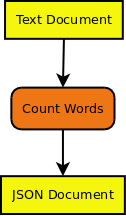
\includegraphics[height=6cm]{images/WpsInOut.png}
  %       \end{figure}
  %     \end{column}
  %   \end{columns}
  % \end{frame}

%------------------------------------------------

  % \begin{frame}[plain]
  %   \frametitle{Example: WPS Chain}
  %   \begin{figure}
  %     \includegraphics[height=6cm]{images/WpsChain.png}
  %   \end{figure}
  % \end{frame}

%------------------------------------------------

  \section{Birdhouse Components}

%------------------------------------------------

  \begin{frame}[plain]
    \frametitle{Birdhouse Components}
    \begin{figure}
      \begin{center}
        \includegraphics[width=11.5cm]{images/birdhouse-components.png}
      \end{center}
    \end{figure}
  \end{frame}

%------------------------------------------------

  \begin{frame}
    \frametitle{Phoenix web-based WPS client}
    \begin{figure}
      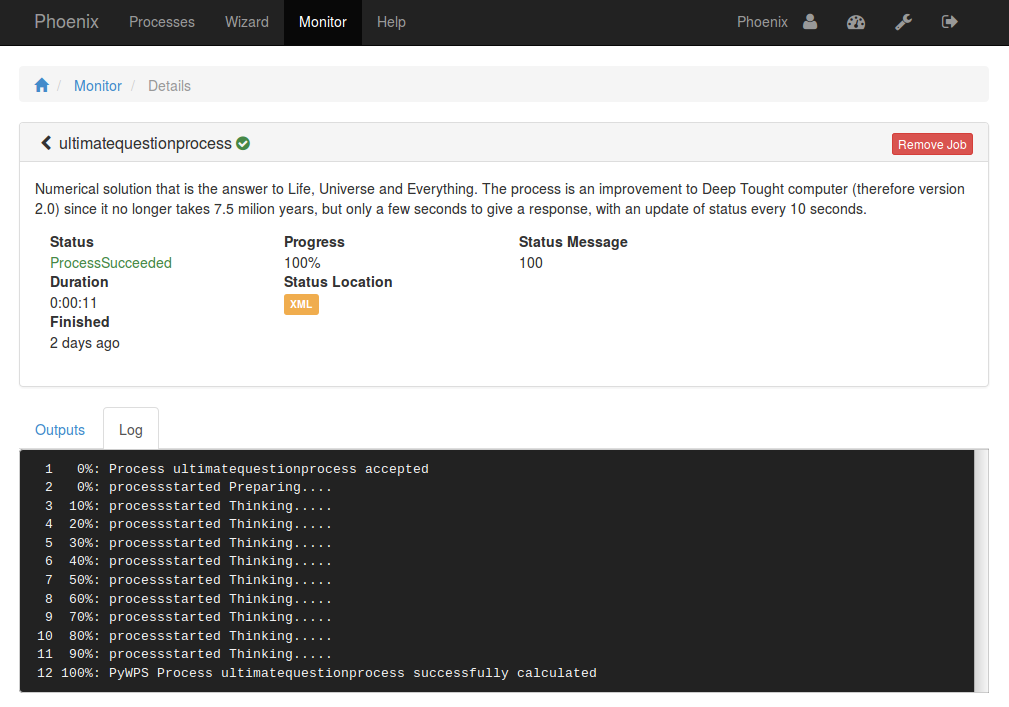
\includegraphics[width=11.5cm]{images/phoenix.png}
    \end{figure}
  \end{frame}

%------------------------------------------------

  \begin{frame}[fragile]
    \frametitle{Birdy command line WPS client}
    \begin{verbatim}
>> conda install -c birdhouse birdhouse-birdy
>> export WPS_SERVICS=http://localhost:8094/wps
>> birdy -h
    \end{verbatim}
    \begin{figure}
      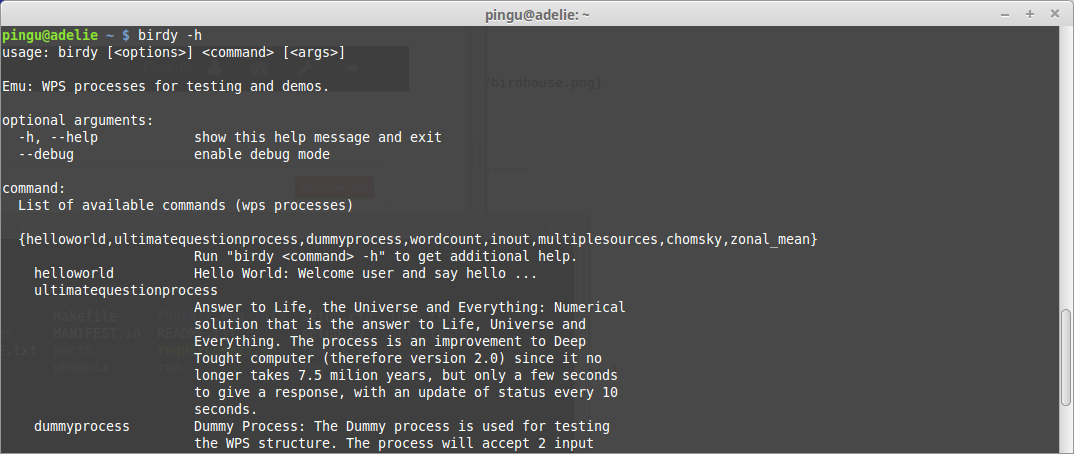
\includegraphics[width=11.5cm]{images/birdy-terminal.png}
    \end{figure}
\end{frame}

%------------------------------------------------

  \begin{frame}
    \frametitle{Birdhouse WPS serivces}
    \begin{itemize}
      \item Malleefowl (for internal use): download data with cache, workflows ...
      \item Emu: processes for testing and demo
      \item Hummingbird: processes for general tools used in the climate science community like cdo and cfchecker
      \item Flyingpigeon: processes for climate data, indices and extreme events
    \end{itemize}
  \end{frame}


%------------------------------------------------

  \begin{frame}
    \frametitle{WSGI Application controlled with Supervisor}
    \begin{figure}
      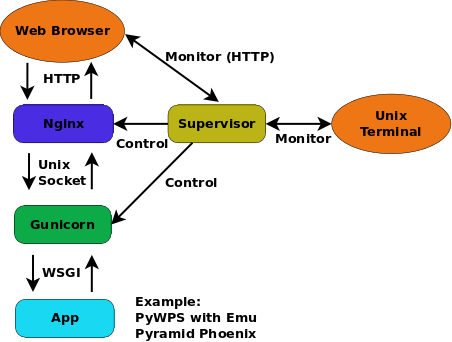
\includegraphics[width=8cm]{images/WsgiApp.png}
    \end{figure}
  \end{frame}

%------------------------------------------------

  \begin{frame}
    \frametitle{Workflow Process in Birdhouse}
    \begin{itemize}
      \item the chain of WPS processes is controlled by a Workflow Engine (dispel4py) 
      \item The Workflow Process itself is a WPS process
      \item data-search, download and publish are internal processes (provided by Malleefowl)
      \item Compute is a process choosen by the user ... for example cfchecker
      \item The Phoenix wizard is used to collect the parameters for the workflow process
    \end{itemize}
    \begin{figure}
      \includegraphics[width=11.5cm]{images/WpsWorkflow.png}
    \end{figure}
  \end{frame}

%------------------------------------------------

  \section{Birdhouse Builder}

%------------------------------------------------

  \begin{frame}
    \frametitle{Why Conda and Buildout?}
    \begin{itemize}
      \item many components: WPS, WMS, web-server, solr, ...
      \item lots of dependencies: cdo, cfchecker, ocgis, numpy, R, ...
      \item many different kinds of config files need to be configured 
      \item installation needs to be reproducible at different locations
      \item should work with different Linux distributions (Centos, Fedora, Debian, Ubuntu, ...)
    \end{itemize}
    \begin{figure}
      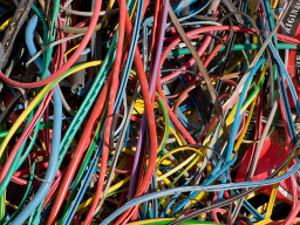
\includegraphics[width=4cm]{images/chaos.png}
    \end{figure}
  \end{frame}

%------------------------------------------------

  \subsection{Conda}

%------------------------------------------------

  \begin{frame}[fragile]
    \frametitle{conda package manager}
    \begin{itemize}
      \item originally for python ... but has a general concept
      \item does not need admin rights
      \item manages dependencies
    \end{itemize}
    \begin{block}{install from birdhouse channel}
      \begin{verbatim}
>> conda install -c birdhouse pywps cdo 
      \end{verbatim}
    \end{block}
    \begin{block}{create conda environment=emu}
      \begin{verbatim}
>> conda create -n emu -c birdhouse \
        python=2.7 cdo pywps 
      \end{verbatim}
    \end{block}
\end{frame}

%------------------------------------------------

  \begin{frame}[fragile]
    \frametitle{conda recipe}
    \begin{block}{meta.yaml}
      \lstinputlisting{meta.yaml}
    \end{block}
    \begin{block}{build conda package}
      \begin{verbatim}
>> ls  
meta.yaml build.sh
>> conda build .
      \end{verbatim}
    \end{block}
\end{frame}

%------------------------------------------------

  \begin{frame}[plain]
    \frametitle{Anaconda Cloud}
    \begin{figure}
      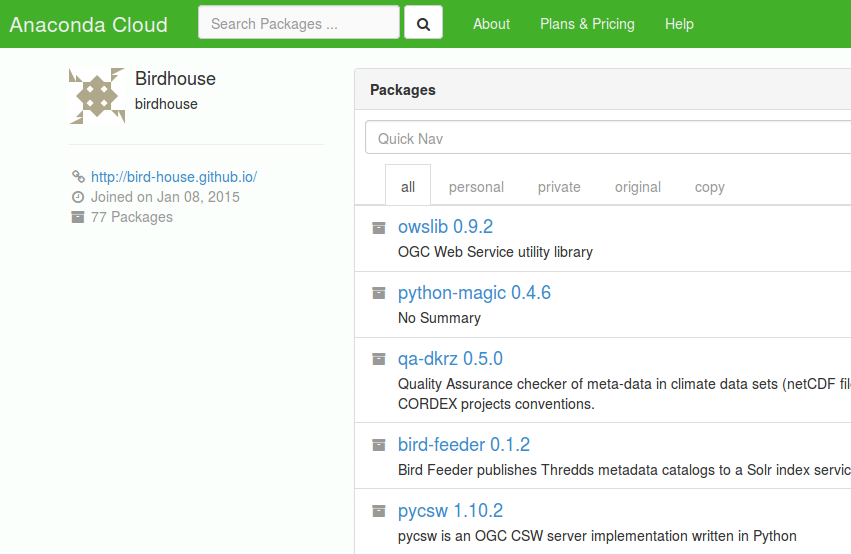
\includegraphics[width=11.5cm]{images/anaconda-cloud.png}
    \end{figure}
  \end{frame}

%------------------------------------------------

  \subsection{Buildout}

%------------------------------------------------

  \begin{frame}
    \frametitle{Buildout}
    \begin{itemize}
      \item Python based build system
      \item creates application with multiple components including configuration files
      \item works also for non-Python parts
      \item using a buildout configuration 
      \item can be extended with recipes
    \end{itemize}
  \end{frame}

%------------------------------------------------

  \begin{frame}[fragile]
    \frametitle{Buildout configuration}
    \begin{block}{buildout.cfg}
      \lstinputlisting{buildout.cfg}
    \end{block}
\end{frame}

%------------------------------------------------

  \begin{frame}[fragile]
    \frametitle{Buildout Recipe}
    \begin{block}{birdhousebuilder.recipe.pywps}
      \lstinputlisting{recipe.py}
    \end{block}
\end{frame}

%------------------------------------------------

  \begin{frame}[fragile]
    \frametitle{Install Birdhouse Component with Buildout}
    \begin{itemize}
      \item for convienience there is a Makefile to call the buildout commands
      \item all Birdhouse components (WPS, Phoenix) are installed in the same way
    \end{itemize}
    \begin{block}{First installation}
      \begin{verbatim}
>> git clone https://github.com/bird-house/emu.git  
>> cd emu
>> make clean install
>> make start
      \end{verbatim}
    \end{block}
\begin{block}{Update configuration like hostname, port}
      \begin{verbatim}
>> vim custom.cfg   
>> make update
>> make restart
      \end{verbatim}
    \end{block}
\end{frame}

  \section{Deployment with Docker}

%------------------------------------------------

  \begin{frame}
    \frametitle{What is Docker?}
    \begin{itemize}
      \item a lightweight Virtual-Machine using Linux Containers
      \item isolated environment for your Linux installation
      \item runs on the same hardware as the host
      \item run latest Ubuntu on an older Centos
      \item rapid startup time
      \item only changed parts of docker image need to loaded on update
    \end{itemize}
    \begin{figure}
      
\includegraphics[width=4cm]{images/docker-container.png}
    \end{figure}
  \end{frame}

%------------------------------------------------

  \begin{frame}
    \frametitle{Containers vs VMs (slide taken from docker)}
    \begin{figure}
      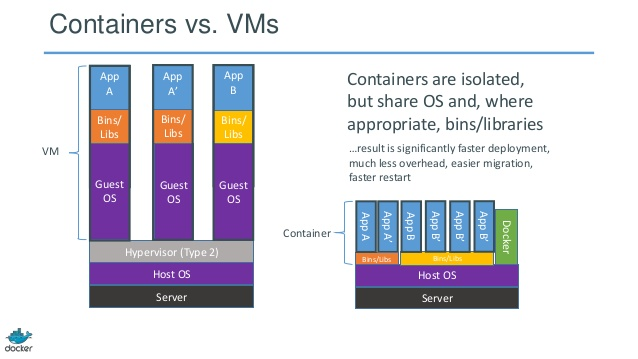
\includegraphics[width=11.5cm]{images/docker-vs-vms.jpg}
    \end{figure}
  \end{frame}

%------------------------------------------------

  \begin{frame}[plain]
    \frametitle{Deploy Birdhouse with Docker}
    \begin{itemize}
      \item each service is running in a Docker container
      \item docker containers can be \emph{linked} to other containers
      \item only some containers (Phonix, WPS Proxy) need to be exposed to external use
    \end{itemize}
    \begin{figure}
      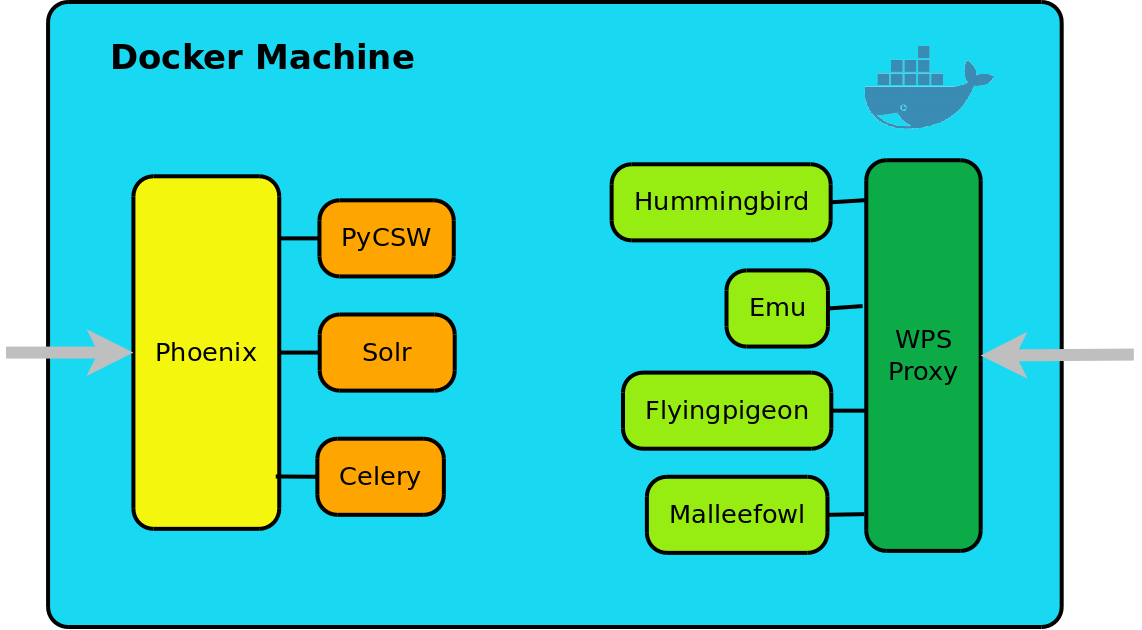
\includegraphics[width=10cm]{images/BirdhouseDocker.png}
    \end{figure}
  \end{frame}

%------------------------------------------------

  \begin{frame}[fragile,shrink]
    \frametitle{Dockerfile}
    \lstinputlisting{Dockerfile}
\end{frame}

%------------------------------------------------

  \begin{frame}[fragile,shrink]
    \frametitle{Try a Docker ...}
    \begin{block}{Images are available on DockerHub}
      \url{https://hub.docker.com/u/birdhouse/}
    \end{block}
    \begin{block}{Start a docker image with Emu WPS}
      \begin{verbatim}
>> docker run -it -p 8090:8090 -p 8094:8094 \
         --name=emu_wps birdhouse/emu  
      \end{verbatim}
    \end{block}
    \begin{block}{Run WPS GetCapabilities Request}
      \begin{verbatim}
http://localhost:8094/wps? \
   service=WPS&version=1.0.0&request=getcapabilities
      \end{verbatim}
    \end{block}
\end{frame}

%------------------------------------------------

  \section{Security and Interoperability}

%------------------------------------------------

  \begin{frame}
    \frametitle{WPS Security Proxy (planned)}
    \begin{itemize}
      \item using string token (uuid) as part of URL to protect WPS execute access
      \item X509 certificates to access (remote) data from ESGF are provided by proxy (using environ)
      \item implemented as WSGI application layer
    \end{itemize}
    \begin{figure}
      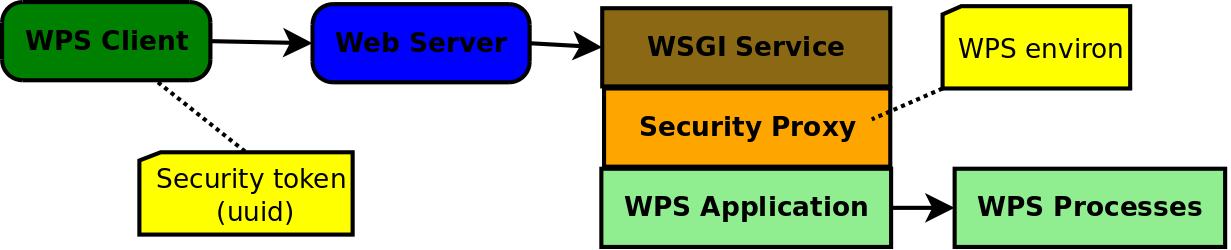
\includegraphics[width=11.5cm]{images/WpsProxy.png}
    \end{figure}
  \end{frame}

  \begin{frame}
    \frametitle{Best Practises to make WPS interchangeable}
    \begin{itemize}
      \item support of complete WPS protocol (literal type, complex types, ...)
      \item separation of WPS definition and functional code (provided as Python library)
      \item convenience and integration code provided as library (e.a. Malleefowl provides functions used by WPS processes)
      \item using WPS profiles (common WPS process definitions)
      \item use self-describing possibilities of WPS
      \item parameters relevant for the process should be part of the process definition
    \end{itemize}
  \end{frame}

%------------------------------------------------

  \appendix

  \section{Appendix}
  
   \begin{frame}[allowframebreaks]
    \frametitle<presentation>{Further Reading}    
    \begin{thebibliography}{10}    
      \beamertemplatearticlebibitems
    \bibitem{birdhouse}
      Birdhouse
      \newblock \url{http://bird-house.github.io/}
    \bibitem{buildout}
      Buildout
      \newblock \url{http://www.buildout.org/}
    \bibitem{anaconda}
      Anaconda
      \newblock \url{https://www.continuum.io/why-anaconda}
    \bibitem{foos4g-ebrahim}
      Evaluation of WPS Frameworks
      \newblock \url{http://www.slideshare.net/mepa1363/foss4g-ebrahim}
    \bibitem{wps-cct}
      Web Processing Service
      \newblock http://www.slideshare.net/GasperiJerome/20130530-web-processing-service-cct-cloud-toulouse-29423710
   
    \end{thebibliography}
    
  \end{frame}
  
%------------------------------------------------

  \begin{frame}
    \Huge{\centerline{The End}}
  \end{frame}

%------------------------------------------------

\end{document}
